\textbf{3.} We roll a die.  If five dots show, we flip on an oscillator that generates $X(t) = \sin (2 \pi t)$ volts.  Otherwise, we turn on a one volt DC (constant) power supply and get $X(t)=1$.
  \begin{enumerate}
  \item  What is the expected value of $X(t)$ at $t=1$?\\
    \textbf{Answer:}\\
    $\sin(2\pi) = 0$, so $E[X(t=1)] = 0 * \frac{1}{6} + 1* \frac{1}{6} + 1* \frac{1}{6}  + 1* \frac{1}{6}  + 1* \frac{1}{6}  + 1* \frac{1}{6}  = \frac{5}{6}$ $\hfill\blacksquare$\\

  \item  What is the variance of $X(t)$ at $t=1$?\\
    \textbf{Answer:}\\
    \begin{align*}
      \sigma^2 & = E[X^2(t=1)] - E[X(t=1)]^2\\
               & = 0^2 * \frac{1}{6} + 1^2* \frac{1}{6} + 1^2* \frac{1}{6}  + 1^2* \frac{1}{6}  + 1^2* \frac{1}{6}  + 1^2* \frac{1}{6} - \left(\df{5}{6}\right)^2 \\
               & = \df{5}{6} - \df{25}{36} = \df{5}{36}
    \end{align*} $\hfill\blacksquare$

  \item  What is the cumulative distribution, $F_X (x)$, of $X(t)$ at $t=1$?\\
    \textbf{Answer:}\\
    Plot is shown in figure~\ref{fig:prob3c} $\hfill\blacksquare$
    \begin{figure}[!h]
      \begin{center}
        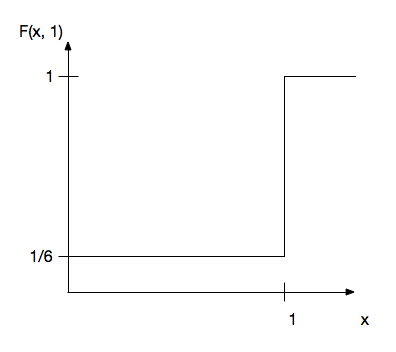
\includegraphics[width=5in]{pics/problem3(c).png}
      \end{center}
      \caption{C.D.F. of $F(x, 1)$}
      \label{fig:prob3c}
    \end{figure}
  \item  Are there any values of $t$ where $X(t)$ is deterministic?\\
    \textbf{Answer:}\\
    Yes, when $t = \frac{1}{4} + k$ where $k \in \mathbb{N}$, $X(t) = 1$, since for both cases,
    the outcome is 1. $\hfill\blacksquare$
    % \item  Is $X(t)$ ergodic?\footnote{No math is required. Just an explanation.}
  \end{enumerate}

